\PassOptionsToPackage{unicode}{hyperref}
\documentclass[aspectratio=1610, professionalfonts, 9pt, hyperref={colorlinks=false}]{beamer}

\usefonttheme[onlymath]{serif}
\usetheme[showtotalframes]{tudo}

\ifluatex
  \usepackage{polyglossia}
  \setmainlanguage{german}
\else
  \ifxetex
    \usepackage{polyglossia}
    \setmainlanguage{german}
  \else
    \usepackage[german]{babel}
  \fi
\fi
    

% Mathematik
\usepackage{amsmath}
\usepackage{amssymb}
\usepackage{mathtools}
\usepackage{cancel}


\usepackage{hyperref}

\usepackage{bookmark}

% Biber
\usepackage[style=numeric-comp,backend=bibtex,sorting=none]{biblatex}
\addbibresource{references.bib}
\DefineBibliographyStrings{german}{andothers = {{et\,al\adddot}}}

% SI UNITX

\usepackage[
  locale=DE,                 % deutsche Einstellungen
  separate-uncertainty=true, % immer Fehler mit \pm
  per-mode=reciprocal,       % ^-1 für inverse Einheiten
  % alternativ:
  % per-mode=reciprocal, % m s^{-1}
  % decimal-marker=., % . statt , f�r Dezimalzahlen
]{siunitx}

%%%%%%%%%%%%%%%%%%%%%%%%%%%%%%%%%%%%%%%%%%%%%%%%%%%%%%%%%%%%%%%%%%%%%%%%%%%%%%%%
%%%%%-------------Hier Titel/Autor/Grafik/Lehrstuhl eintragen--------------%%%%%
%%%%%%%%%%%%%%%%%%%%%%%%%%%%%%%%%%%%%%%%%%%%%%%%%%%%%%%%%%%%%%%%%%%%%%%%%%%%%%%%

%Titel:
\title{Von der Entdeckung der kosmischen Strahlung bis zu modernen Luftschauerexperimenten}
%Autor
\author[J.~Alameddine]{Jean-Marco Alameddine}
%Lehrstuhl/Fakultät
\institute[Lehrstuhl E5b]{Lehrstuhl E5b \\  Fakultät Physik}
%Titelgrafik 
%\titlegraphic{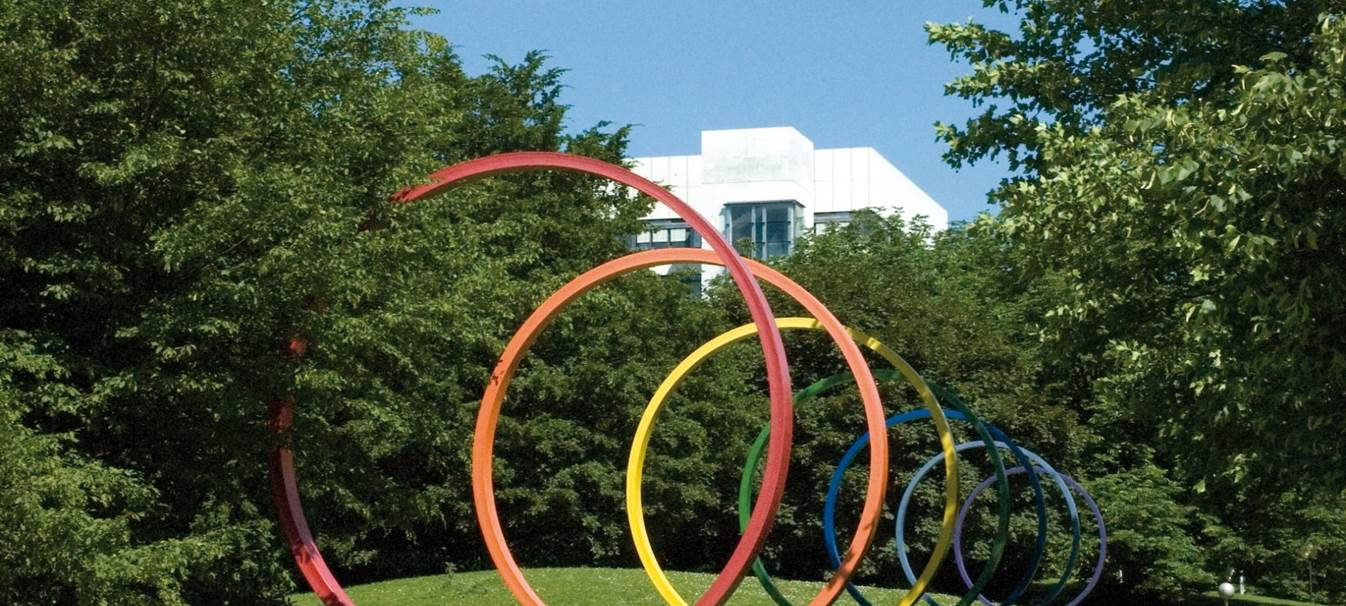
\includegraphics[width=0.7\textwidth]{images/tudo-title-2.jpg}}


\begin{document}

\maketitle



\begin{frame}
    Ende 19. Jahrhundert: "Die Physik ist als Wissenschaft abgeschlossen..."
    \begin{figure}
        \includegraphics<2>[width=0.23\textwidth]{images/first_xray.jpg} 
        \only<2->{\cite{xray}}
        \hfill
        \includegraphics<2>[width=0.4\textwidth]{images/Becquerel_plate.jpg} 
        \only<2->{\cite{radio}}
        \hfill
        \includegraphics<2>[width=0.23\textwidth]{images/Max_Planck_(1858-1947).jpg}
        \only<2->{\cite{planck}}
    \end{figure}
\end{frame} 


\begin{frame}{Der Weg zur kosmischen Höhenstrahlung...}
  \begin{columns}
    \column{0.6\textwidth}
      \begin{itemize}
        \setlength\itemsep{0.5em}
        \item Bereits früh bekannt (Coulomb, 1785): Ein isolierter elektrischer Leiter verliert mit der Zeit seine Ladung
        \item [$\rightarrow$] Leitfähigkeit der Luft?
        \item Elster und Geitel (siehe Abbildung) 1900 mit der Hypothese:
        \item [$\rightarrow$] Kleinste Mengen radioaktiver Substanzen in der Luft und in der Erde, welche der Luft ihre Leitfähigkeit verleihen
        \item Erste Untersuchungen von Ionisation außerhalb von Laboren (Höhlen, Salzminen...)
      \end{itemize}
        \vspace*{10px}
  
    \column{0.4\textwidth}
      \begin{figure}
          \centering
          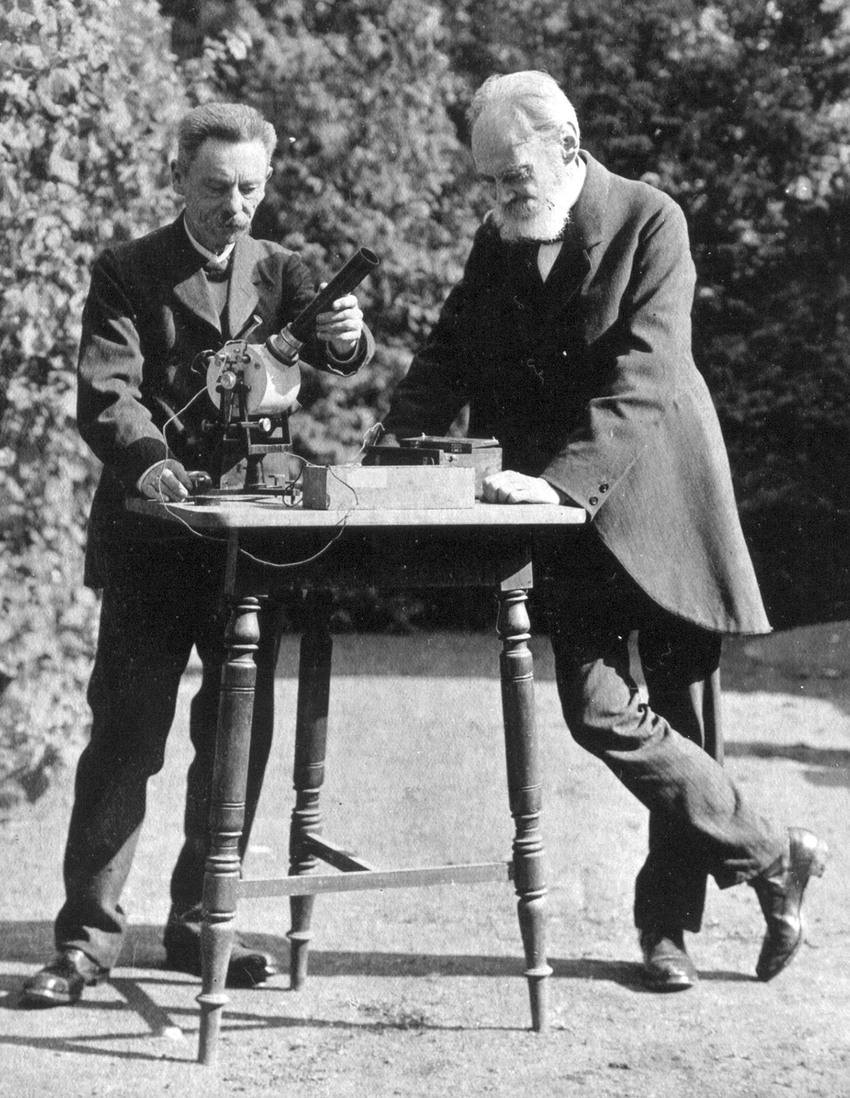
\includegraphics[width=0.7\linewidth]{images/Julius-Elster-and-Hans-Geitel-experimenting-in-the-garden-of-Elsters-house-The.png}
          \caption{Julius Elster und Hans Geitel \cite{article}}
      \end{figure}
  \end{columns}
\end{frame}

\begin{frame}{Erste Untersuchungen der Ionisation in der Höhe}
      \begin{itemize}
        \setlength\itemsep{0.5em}
        \item Erste Messungen der Ionisation (mithilfe eines Elektroskopes) in der Höhe:
        \item[$\rightarrow$] \textbf{1910}: Theodor Wulf, Messung auf dem Eiffelturm ($h \approx \SI{300}{\metre}$)  
        \item[$\rightarrow$] \textbf{1909-1911}: Albert Gockel, Ballonflüge in der Schweiz ($h \lesssim \SI{4500}{\metre}$)
      \end{itemize}
        \vspace*{10px}

        $\Rightarrow$ Deutlich geringere Abnahme der Ionisationsstärke mit der Höhe als angenommen 
\end{frame}

\begin{frame}{}
  \begin{columns}
    \column{0.5\textwidth}
      \begin{itemize}
        \setlength\itemsep{0.5em}
        \item Victor Hess, arbeitete ab 1910 am "Institut für Radiumforschung" in Wien
        \item Durchmessung von Untersuchungen der Absorption von \gamma-Strahlung in Luft
        \item [$\rightarrow$] Schlussfolgerung aus Messungen: In \SI{500}{\metre} Höhe würde die Strahlung der Erde auf wenige Prozent abgefallen sein
      \end{itemize}
        \vspace*{10px}
  
    \column{0.5\textwidth}
      \begin{figure}
          \centering
          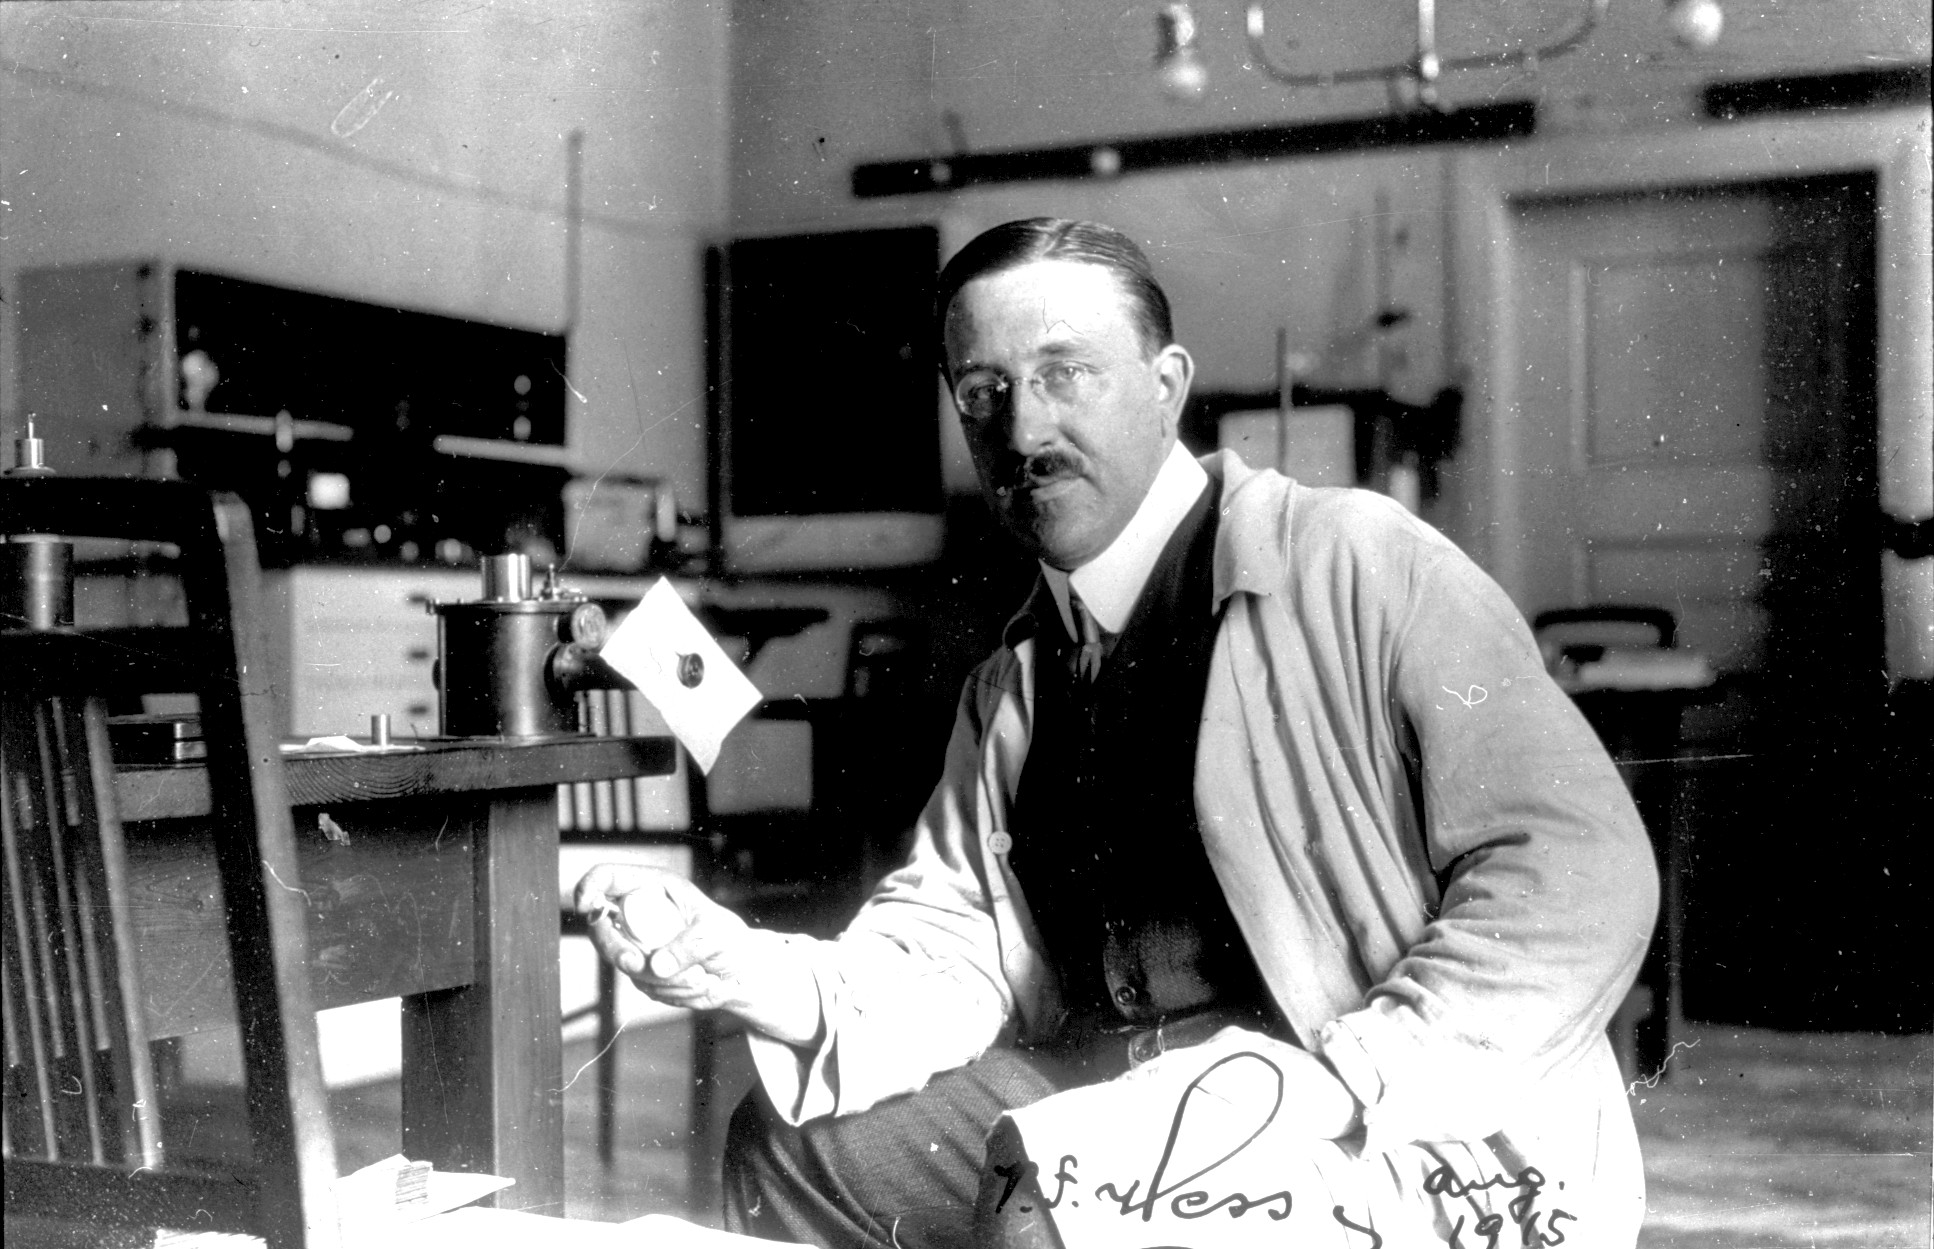
\includegraphics[width=\linewidth]{images/X-HESS-2140.jpg}
          \caption{Viktor Hess im Jahre 1915 \cite{hess}}
      \end{figure}
  \end{columns}
\end{frame}


\begin{frame}{}
  \begin{columns}
    \column{0.5\textwidth}
      \begin{itemize}
        \setlength\itemsep{0.5em}
        \item \textbf{1911}: Erste Ballonflüge durch Hess 1911 ($h \approx \SI{1000}{\metre}$)
        \item [$\rightarrow$] Bestätigung der Resultate von Gockel
        \item \textbf{1912, erste Hälfte}: Sechs weitere Ballonflüge, zu verschiedenen Tagszeiten ($h \lesssim \SI{2100}{\metre}$)
        \item [$\rightarrow$] Keine Korrelation der Ionsationrate mit Sonnenaktivitäten
        \item [$\rightarrow$] Bestätigung: Ionisatonsrate nimmt nicht signifikant stark mit der Distanz zur Erde ab
      \end{itemize}
        \vspace*{10px}

    Ziel von Hess: Untersuchung der Ionsationsrate in größeren Höhen
  
    \column{0.5\textwidth}
      \begin{figure}
          \centering
          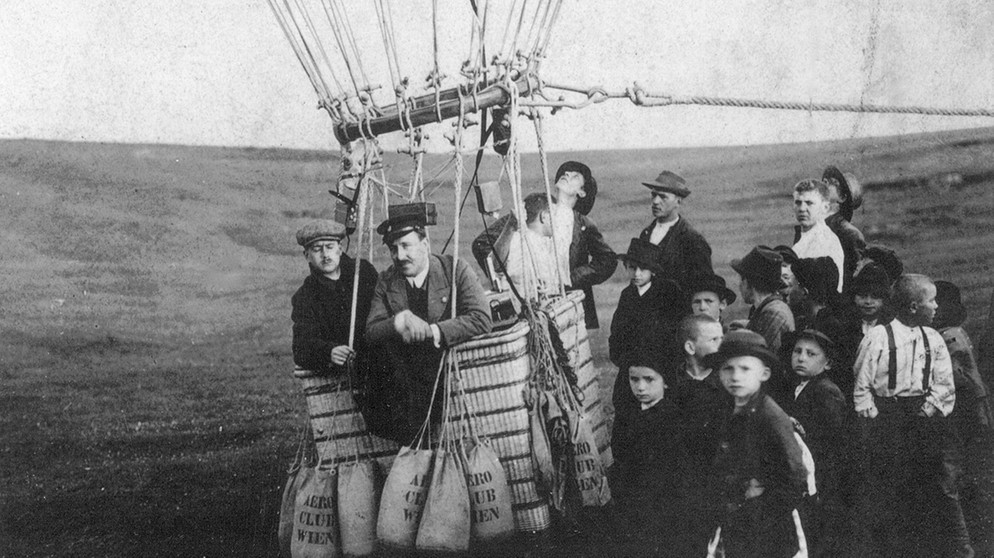
\includegraphics[width=\linewidth]{images/ballon.jpg}
          \caption{Victor Hess in einem Ballon um 1912 \cite{baloon}}
      \end{figure}
  \end{columns}
\end{frame}


\begin{frame}{}
  \begin{columns}
    \column{0.5\textwidth}
      \begin{itemize}
        \setlength\itemsep{0.5em}
        \item \textbf{7. August 1912}: Ballonflug von Hess auf bis zu $h \approx \SI{5350}{\metre}$
        \item [$\rightarrow$] Gemessener Anstieg der Ionisationsrate von $h \approx \SI{3000}{\metre}$ auf $h \approx \SI{5200}{\metre}$ um Faktor vier!
        \item [$\rightarrow$] Hess: Es muss sich um eine durchgringende Strahlung handeln, die die Atmosphäre von oben trifft (und nicht von der Sonne stammt)
        \item \textbf{1913, 1914}: Bestätigung der Ergebnisse, Ballonflüge von Werner Kolhörster ($h \approx \SI{9300}{\metre}$)
      \end{itemize}


      \begin{itemize}
        \item Anfangs bestand bei vielen Forschern Zweifel, dass die entdeckte Strahlung tatsächlich kosmischen Ursprunges war
      \end{itemize}

    \column{0.5\textwidth}

      \begin{figure}
          \centering
          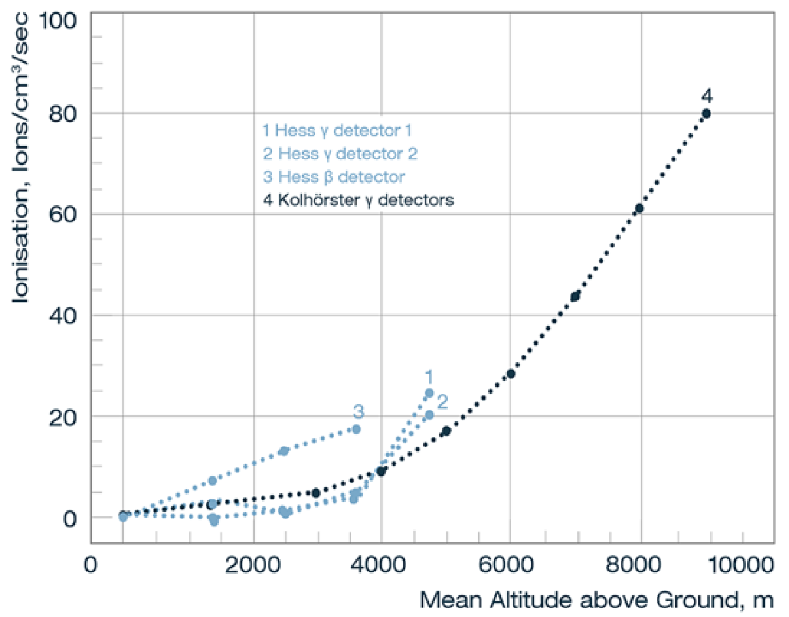
\includegraphics[width=\linewidth]{images/walter2.png}
          \caption{Ergebnisse des siebten Ballonfluges von Hess und des Ballonfluges von Kolhörster \cite{Hess:2018twh}}
      \end{figure}
  \end{columns}
\end{frame}


% Wenn mir ein gutes Bild zu den Folien über den Weg läuft...
%\begin{frame}{Die Identifikation als Teilchenstrahlung}
%  \begin{columns}
%    \column{0.5\textwidth}
%      \begin{itemize}
%        \setlength\itemsep{0.5em}
%        \item Große Durchdringtiefe der kosmischen Strahlung $\Rightarrow$ Identifikation als \gamma-Strahlung
%        \item Kolhörster: Absorptionskoeffizient der kosmischen Strahlung in Luft um Faktor \num{4.4} kleiner als Koeffizient von bekannten radioaktiven Quellen  
%        \item [$\rightarrow$] Härteres Spektrum?
%        \item Andere experimentelle Methoden lösten Elektrometer ab:
%        \item [$\rightarrow$] Nebelkammer (1911, Wilson)
%        \item [$\rightarrow$] Geiger-Müller-Zählrohr (1928, Geiger, Müller)
%      \end{itemize}
%  
%    \column{0.5\textwidth}
%      \begin{figure}
%          \centering
%          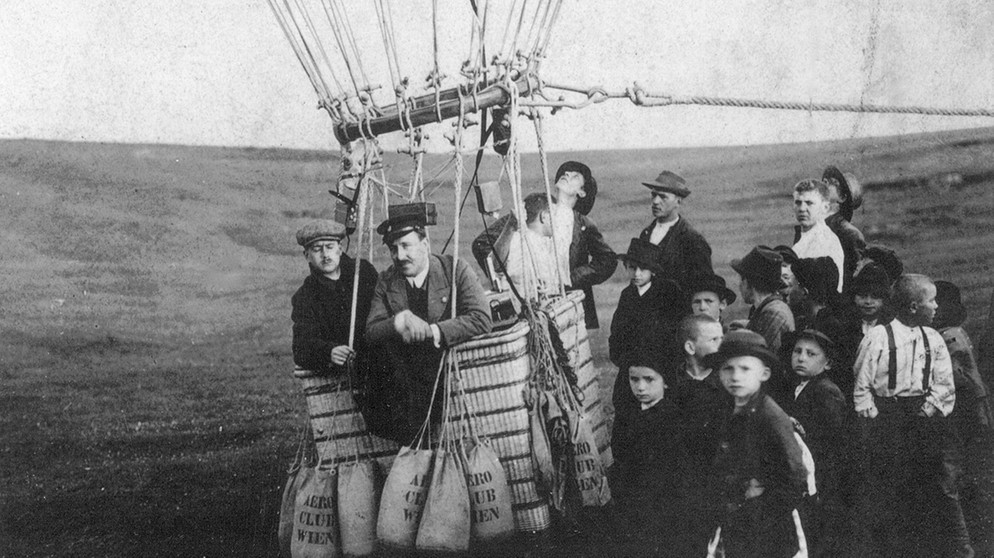
\includegraphics[width=\linewidth]{images/ballon.jpg}
%          \caption{Victor Hess in einem Ballon um 1912 \cite{baloon}}
%      \end{figure}
%  \end{columns}
%\end{frame}

\begin{frame}{Die Identifikation als Teilchenstrahlung}
      \begin{itemize}
        \setlength\itemsep{0.5em}
        \item Große Durchdringtiefe der kosmischen Strahlung $\Rightarrow$ Identifikation als \gamma-Strahlung
        \item Kolhörster: Absorptionskoeffizient der kosmischen Strahlung in Luft um Faktor \num{4.4} kleiner als Koeffizient von bekannten radioaktiven Quellen  
        \item [$\rightarrow$] Härteres Spektrum?
        \item Andere experimentelle Methoden lösten Elektrometer ab:
        \item [$\rightarrow$] Nebelkammer (1911, Wilson)
        \item [$\rightarrow$] Geiger-Müller-Zählrohr (1928, Geiger, Müller), Möglichkeit von Koinzidenzmessungen!
      \end{itemize}
\end{frame}


\begin{frame}{Die Identifikation als Teilchenstrahlung - Bothe und Kolhörster}
  \begin{columns}
    \column{0.5\textwidth}
      \begin{itemize}
        \setlength\itemsep{0.5em}
        \item \textbf{1929}: Koinzidenzmessungen von Bothe und Kolhörster mit Geiger-Müller-Zählrohren
        \item [$\rightarrow$] Ziel: Nachweis dass kosmische Strahlung aus \gamma-Strahlung besteht
        \item [$\rightarrow$] Idee: \gamma-Strahlung lösen Elektronen aus, welche beide Koinzidenzen durchqueren
        \item [$\rightarrow$] Beobachte Einfluss eines Absorbers auf die Koinzidenzen
      \end{itemize}
        \vspace*{10px}
  
    \column{0.5\textwidth}
      \begin{figure}
          \centering
          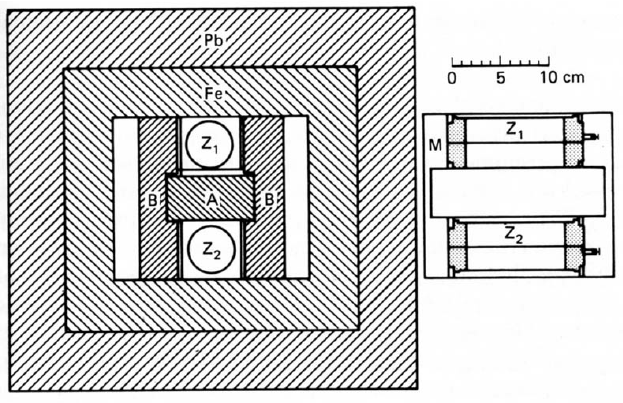
\includegraphics[width=\linewidth]{images/The-experiment-of-Bothe-and-Kolhoerster-in-Ref-48-Coincidences-between-counters-Z-1.png}
          \caption{Experiment von Bothe und Kolhörster \cite{ko}}
      \end{figure}
  \end{columns}
\end{frame}

\begin{frame}{Die Identifikation als Teilchenstrahlung - Bothe und Kolhörster}
  \begin{columns}
    \column{0.5\textwidth}
      \begin{itemize}
        \setlength\itemsep{0.5em}
        \item Mit \SI{4}{\centi\meter} Goldbarren konnten entgegen der Erwartung nur \SI{25}{\percent} der Koinzidenzen entfernt werden
        \item [$\rightarrow$] Die detektierten Teilchen sind so durchdringend wie die kosmische Strahlung selbst
        \item [$\rightarrow$] Es kann sich nicht um \gamma-Strahlung handeln sondern um geladene Teilchen!
      \end{itemize}
        \vspace*{10px}
  
    \column{0.5\textwidth}
      \begin{figure}
          \centering
          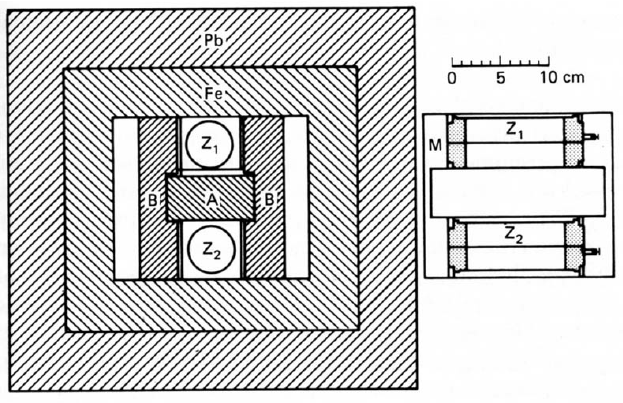
\includegraphics[width=\linewidth]{images/The-experiment-of-Bothe-and-Kolhoerster-in-Ref-48-Coincidences-between-counters-Z-1.png}
          \caption{Experiment von Bothe und Kolhörster \cite{ko}}
      \end{figure}
  \end{columns}
\end{frame}

\begin{frame}{Die Identifikation als Teilchenstrahlung - Breitengradeffekt}
  \begin{columns}
    \column{0.5\textwidth}
      \begin{itemize}
        \setlength\itemsep{0.5em}
        \item \textbf{1919}: Kolhörster: Erster Vorschlag, die Breitengradabhängigkeit der Ionisationsrate zu untersuchen
        \item \textbf{1932, 1933}: Nachweis der Abhängigkeit der Intensität der kosmischen Strahlung vom Breitengrad
        \item [$\rightarrow$] Intensität folgt dem geomagnetischen Feld
        \item [$\rightarrow$] Eindeutiger Nachweis, dass kosmische Strahlung aus geladenen Teilchen besteht
      \end{itemize}
        \vspace*{10px}
  
    \column{0.5\textwidth}
      \begin{figure}
          \centering
          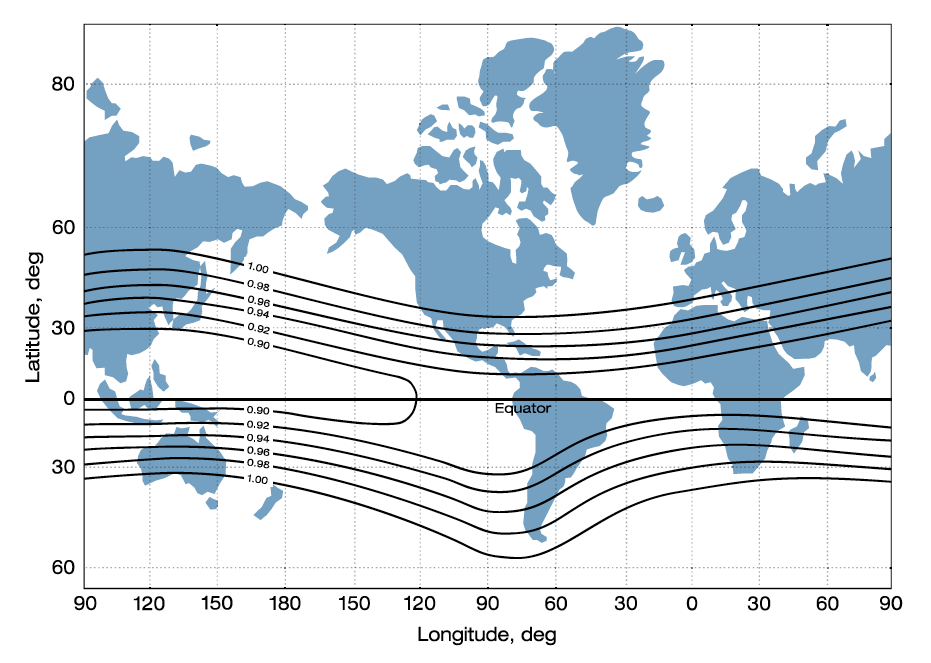
\includegraphics[width=\linewidth]{images/scrrenshot}
          \caption{Breitengradabhängigkeit der kosmischen Strahlung \cite{9789400754225}}
      \end{figure}
  \end{columns}
\end{frame}

\begin{frame}[allowframebreaks]{Quellen}
	\printbibliography

\end{frame}

\end{document}
